    \hypertarget{content-with-notebooks}{%
\section{Content with notebooks}\label{content-with-notebooks}}

You can also create content with Jupyter Notebooks. This means that you
can include code blocks and their outputs in your book.

\hypertarget{markdown-notebooks}{%
\subsection{Markdown + notebooks}\label{markdown-notebooks}}

As it is markdown, you can embed images, HTML, etc into your posts!

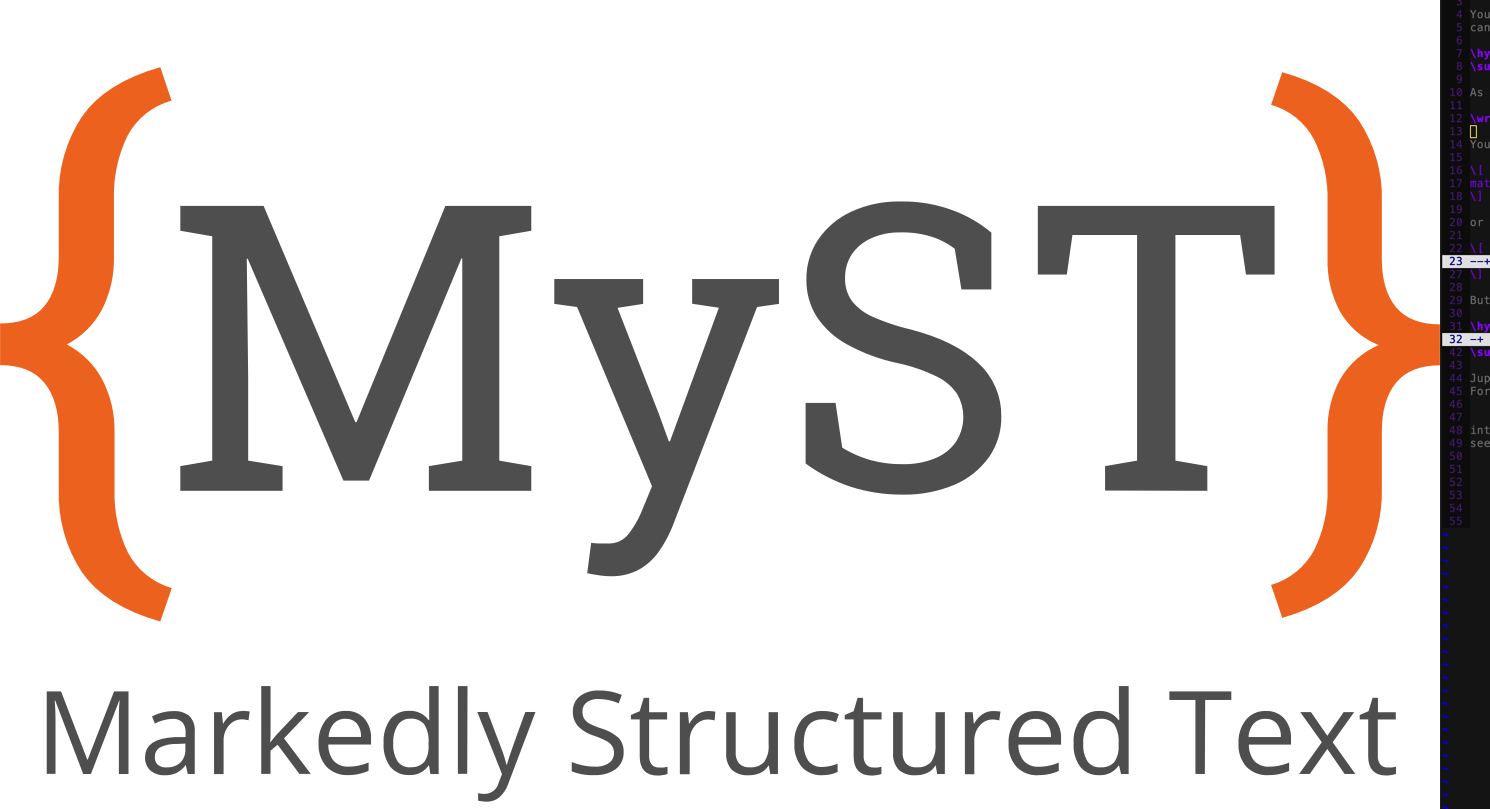
\includegraphics[width=3.5in]{fig/myST.png}

You can also \(add_{math}\) and

\[
math^{blocks}
\]

or

\[
\begin{aligned}
\mbox{mean} la_{tex} \\ \\
math blocks
\end{aligned}
\]

But make sure you \$Escape \$your \$dollar signs \$you want to keep!

\hypertarget{myst-markdown}{%
\subsection{MyST markdown}\label{myst-markdown}}

MyST markdown works in Jupyter Notebooks as well. For more information
about MyST markdown, check out
\href{https://jupyterbook.org/content/myst.html}{the MyST guide in
Jupyter Book}, or see
\href{https://myst-parser.readthedocs.io/en/latest/}{the MyST markdown
documentation}.

\hypertarget{code-blocks-and-outputs}{%
\subsection{Code blocks and outputs}\label{code-blocks-and-outputs}}

Jupyter Book will also embed your code blocks and output in your book.
For example, here's some sample Matplotlib code:

    There is a lot more that you can do with outputs (such as including
interactive outputs) with your book. For more information about this,
see \href{https://jupyterbook.org}{the Jupyter Book documentation}


    % Add a bibliography block to the postdoc
    
    
    
